\section{Results}\label{sec:Results}
\subsection{Spectral Components}
These samples show the effects that can be modeled using the 3D $B_0$ field simulator. In \ref{subfig:without B0}, the spectral peaks have a purely Lorentzian lineshape. In \ref{subfig:some B0}, the lineshape is now Voigtian because the Gaussian term has been added back by the 3D $B_0$ field simulator. In \ref{subfig:with B0}, severe heterogeneities are modeled which produce extremely broad line widths. All three plots use the same x- and y-axes. The observed offsets are caused by the line broadening.


hese samples show how identical spectra are affected by zero- and first-order phase offsets. In \ref{subfig:no phase}, the real component (black) is in absorption mode exhibiting narrow line widths and is fully positive. In \ref{subfig:zero order phase}, a zero-order phase offset is applied. As the spectrum shifts from absorption to dispersion mode, the peaks uniformly lose their symmetry and negative values from the imaginary component are transferred to the real component. In \ref{subfig:first order phase}, a first-order phase shift is applied. This is evident because the asymmetry increases across the spectrum and emanates from the water peak.


These 3 samples show the effect of eddy currents on MRS spectra to various degrees. The strength of the eddy currents increases from \ref{subfig:ec=1} to \ref{subfig:ec=5}. If the time constant, $tc$, is set too long, the eddy current artifact will appear as a global frequency shift. In these examples, it can be seen that only some frequencies are affected.


Examples of 8 simulated coil transients for a 3T GE PRESS sequence with TE=30ms. \ref{subfig:raw transients} shows transients with various SNRs and coil sensitivities along with zero-order phase and frequency offsets. \ref{subfig:phase alignment} shows the transients after phase alignment. \ref{subfig:frequency alignment} shows the transients after frequency alignment. After \ref{subfig:frequency alignment}, the transients can be averaged together and the coil-combined spectrum can then be fitted.

% \begin{figure}[!ht]
    \centering
    \begin{tabular}[c]{ccc}
    \begin{subfigure}[c]{0.31\textwidth}
        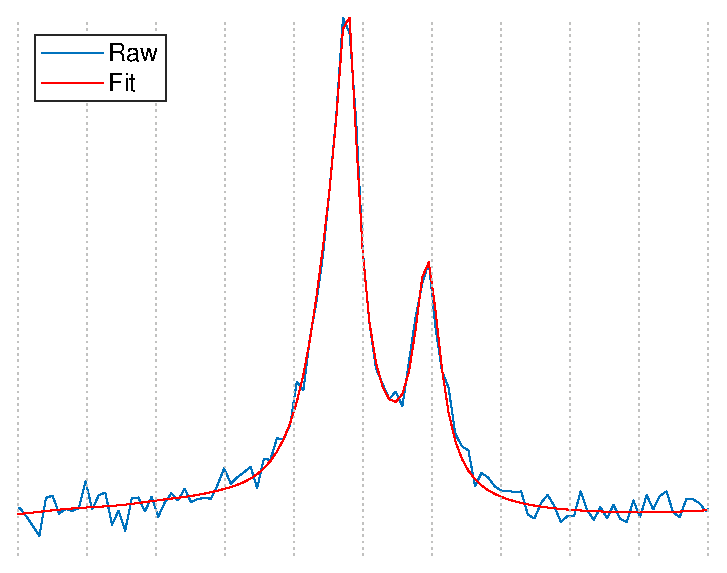
\includegraphics[width=0.95\textwidth,keepaspectratio]{images/b0_peaks/no_B0.eps}
        \caption{Spectral peaks without $B_0$ inhomogeneities ($\mu = 0$Hz)}
        \label{subfig:without B0}
        \vspace{3pt}
    \end{subfigure}&
    \begin{subfigure}[c]{0.31\textwidth}
        \centering
        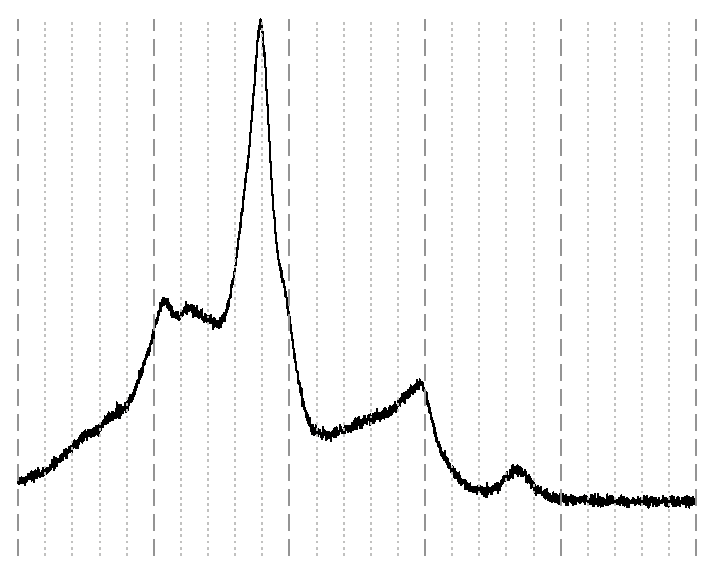
\includegraphics[width=0.95\textwidth,keepaspectratio]{images/b0_peaks/some_B0.eps}
        \caption{Spectral peaks with moderate $B_0$ inhomogeneities ($\mu = 75$Hz)}
        \label{subfig:some B0}      
        \vspace{3pt}
    \end{subfigure}&
    \begin{subfigure}[c]{0.31\textwidth}
        \centering
        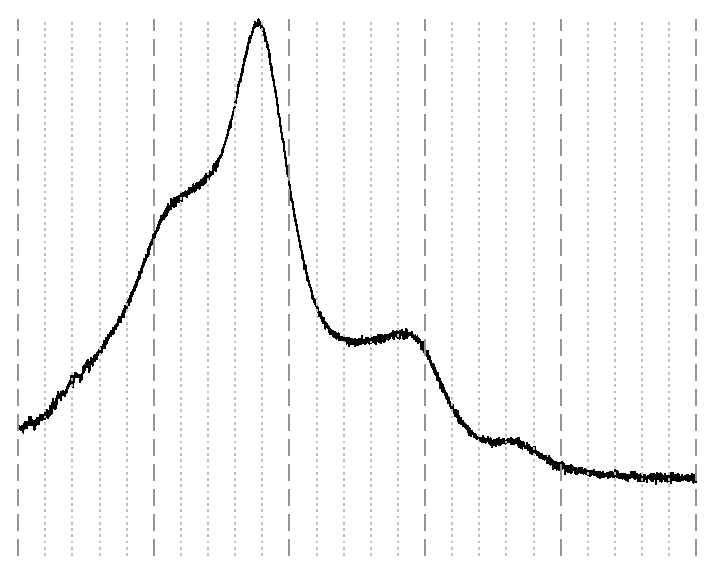
\includegraphics[width=0.95\textwidth,keepaspectratio]{images/b0_peaks/with_B0.eps}
        \caption{Spectral peaks with severe $B_0$ inhomogeneities ($\mu = 175$Hz)}
        \label{subfig:with B0}  
        \vspace{3pt}
    \end{subfigure}\\
    \begin{subfigure}[c]{0.31\textwidth}
        \centering
        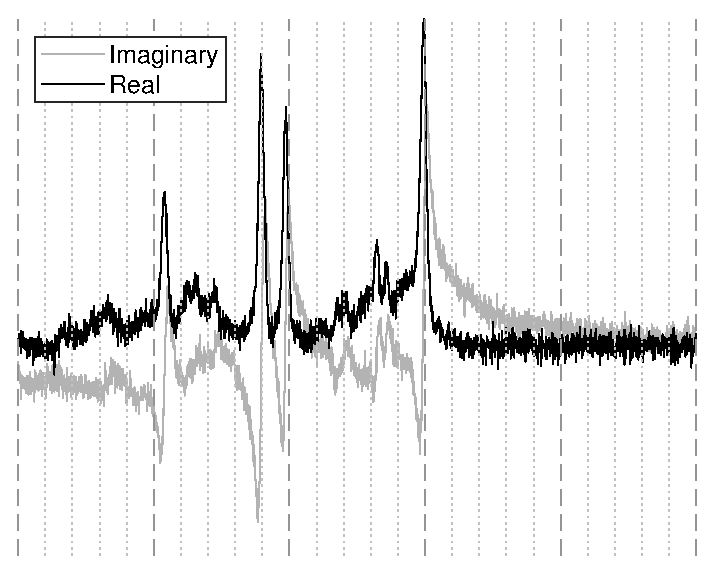
\includegraphics[width=0.95\textwidth,keepaspectratio]{images/phase/no_phase.eps}
        \caption{Spectrum with no phase offsets}
        \label{subfig:no phase}        
        \vspace{3pt}
    \end{subfigure}&
    \begin{subfigure}[c]{0.31\textwidth}
        \centering
        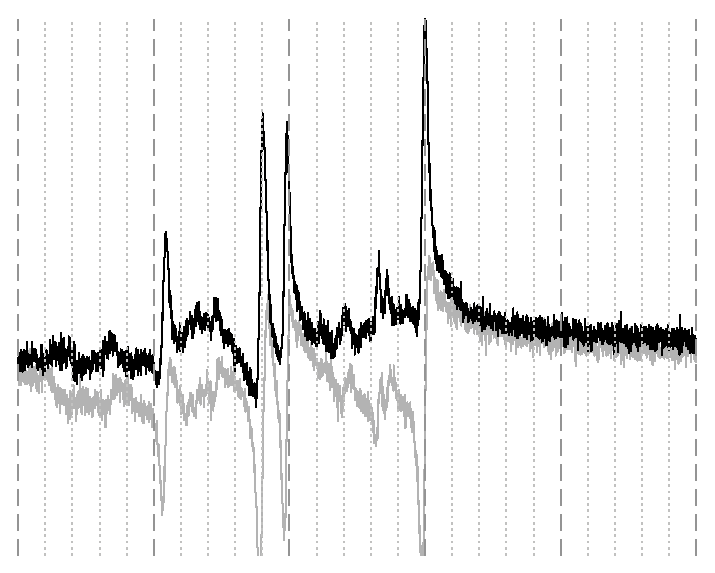
\includegraphics[width=0.95\textwidth,keepaspectratio]{images/phase/zero-order.eps}
        \caption{Spectrum with zero-order phase offset ($\phi_0 = 45^{\circ}$)}
        \label{subfig:zero order phase}        
        \vspace{3pt}
    \end{subfigure}&%
    \begin{subfigure}[c]{0.31\textwidth}
        \centering
        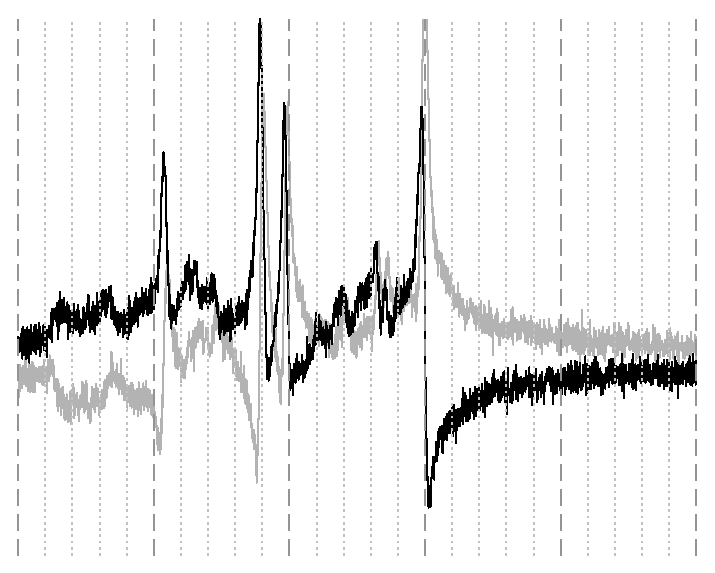
\includegraphics[width=0.95\textwidth,keepaspectratio]{images/phase/first-order.eps}
        \caption{Spectrum with first-order phase offset ($\phi_1 = 20^{\circ}$)}
        \label{subfig:first order phase}        
        \vspace{3pt}
    \end{subfigure}\\
    \begin{subfigure}[c]{0.31\textwidth}
        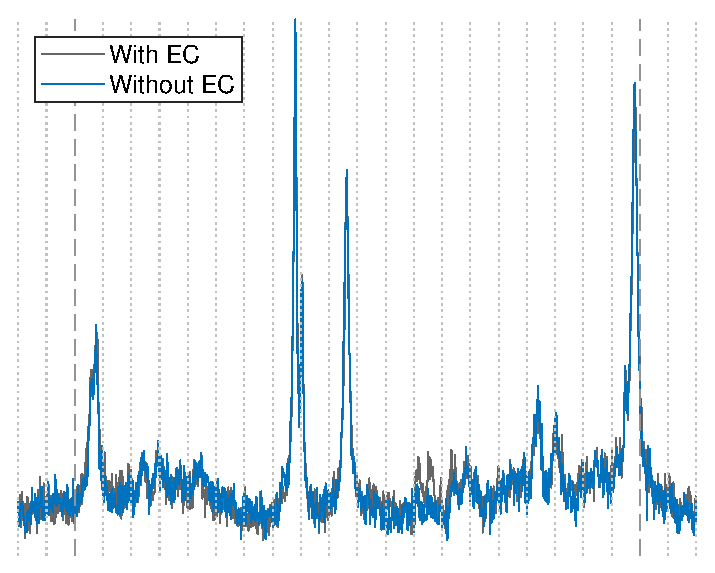
\includegraphics[width=0.95\textwidth, keepaspectratio]{images/eddy/ec=1.eps}
        \caption{Eddy current amplitude = 1.0}
        \label{subfig:ec=1}        
        \vspace{3pt}
    \end{subfigure}&
    \begin{subfigure}[c]{0.31\textwidth}
        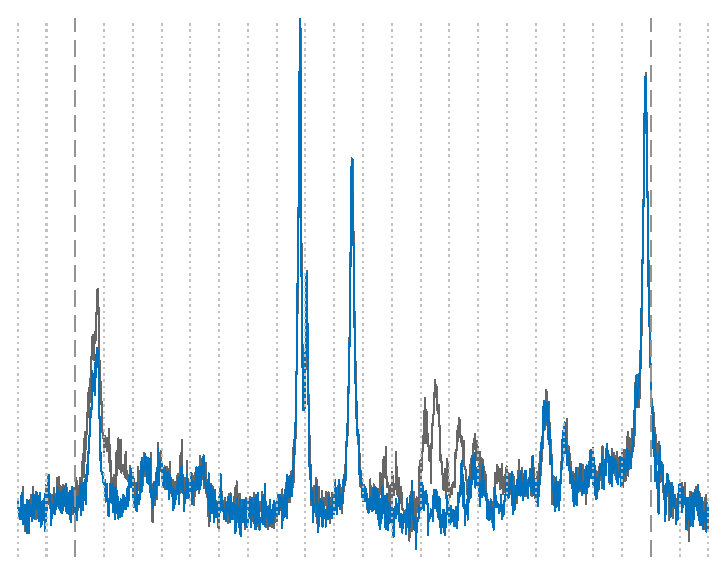
\includegraphics[width=0.95\textwidth, keepaspectratio]{images/eddy/ec=3.eps}
        \caption{Eddy current amplitude = 3.0}
        \label{subfig:ec=3}        
        \vspace{3pt}
    \end{subfigure}&
    \begin{subfigure}[c]{0.31\textwidth}
        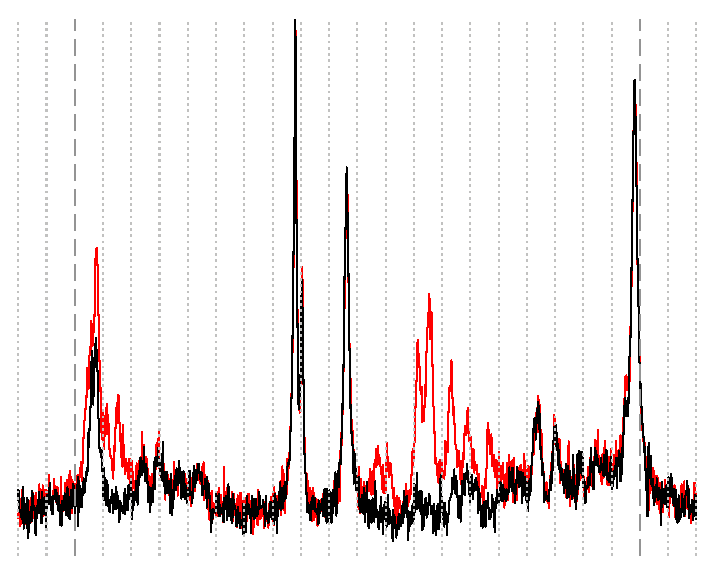
\includegraphics[width=0.95\textwidth, keepaspectratio]{images/eddy/ec=5.eps}
        \caption{Eddy current amplitude = 5.0}
        \vspace{3pt}
    \end{subfigure}\\
    \begin{subfigure}[c]{0.31\textwidth}
        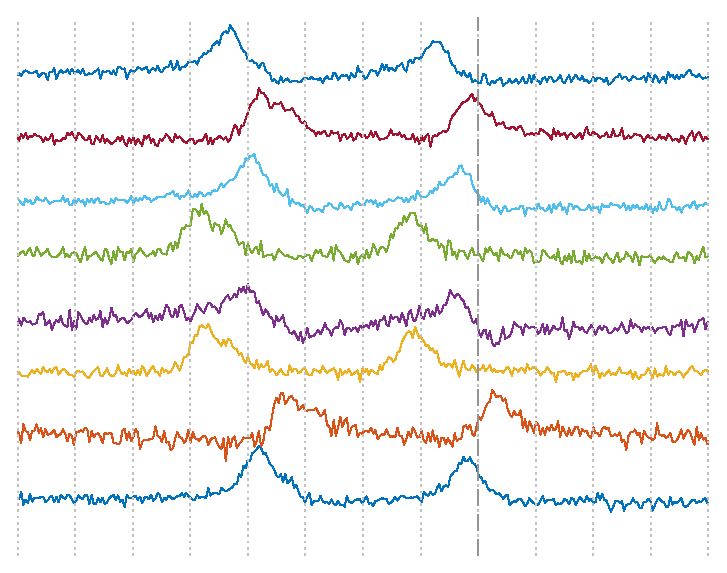
\includegraphics[width=0.95\textwidth, keepaspectratio]{images/samples_transients/8coil_w_phase_w_fshift_cropped.eps}
        \caption{Raw spectral transients}
        \label{subfig:raw transients}      
        \vspace{3pt}
    \end{subfigure}&
    \begin{subfigure}[c]{0.31\textwidth}
        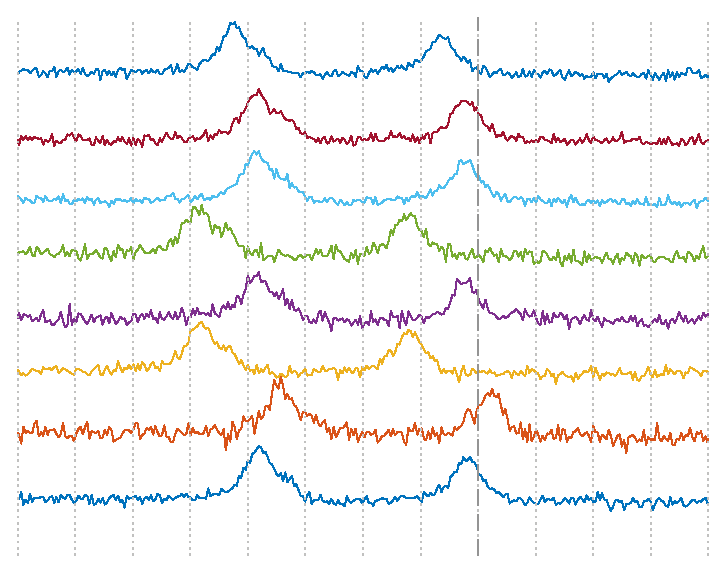
\includegraphics[width=0.95\textwidth, keepaspectratio]{images/samples_transients/8coil_wo_phase_w_fshift_cropped.eps}
        \caption{Phase alignment}
        \label{subfig:phase alignment}        
        \vspace{3pt}
    \end{subfigure}&%
    \begin{subfigure}[c]{0.31\textwidth}
        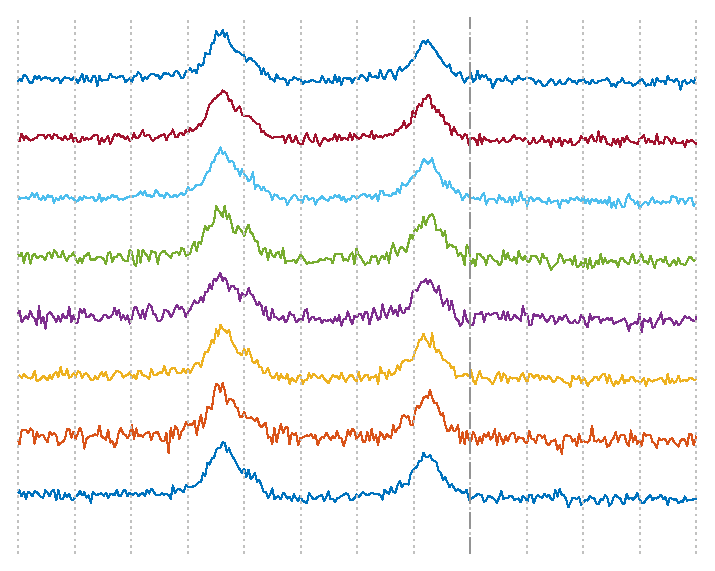
\includegraphics[width=0.95\textwidth, keepaspectratio]{images/samples_transients/8coil_wo_phase_wo_fshift_cropped.eps}
        \caption{Frequency alignment}
        \label{subfig:frequency alignment}      
        \vspace{3pt}
    \end{subfigure}
    \end{tabular}
    \caption{Sample spectra simulated for a PRESS sequence with TE=30ms that highlight the effect of the baseline and residual water contributions.}
    \label{fig:30ms samples curated clean}
\end{figure}


\begin{figure}
    \centering
    \begin{subfigure}{0.32\textwidth}
        \centering
        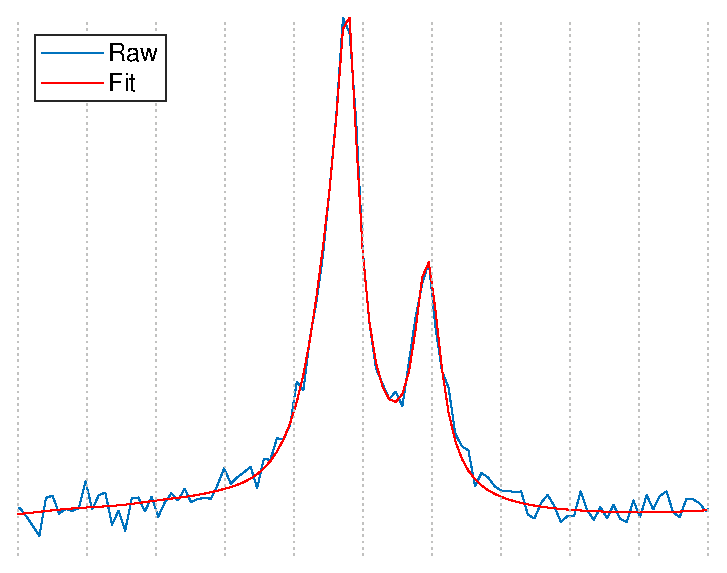
\includegraphics[width=0.95\textwidth,keepaspectratio]{images/b0_peaks/no_B0.eps}
        \caption{Spectral peaks without $B_0$ inhomogeneities ($\mu = 0$Hz)}
        \label{subfig:without B0}        
    \end{subfigure}
    \begin{subfigure}{0.32\textwidth}
        \centering
        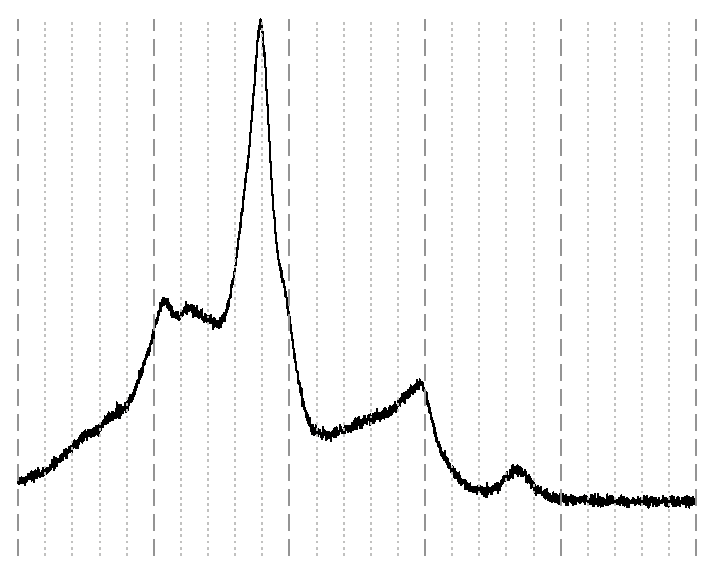
\includegraphics[width=0.95\textwidth,keepaspectratio]{images/b0_peaks/some_B0.eps}
        \caption{Spectral peaks with moderate $B_0$ inhomogeneities ($\mu = 75$Hz)}
        \label{subfig:some B0}        
    \end{subfigure}
    \begin{subfigure}{0.32\textwidth}
        \centering
        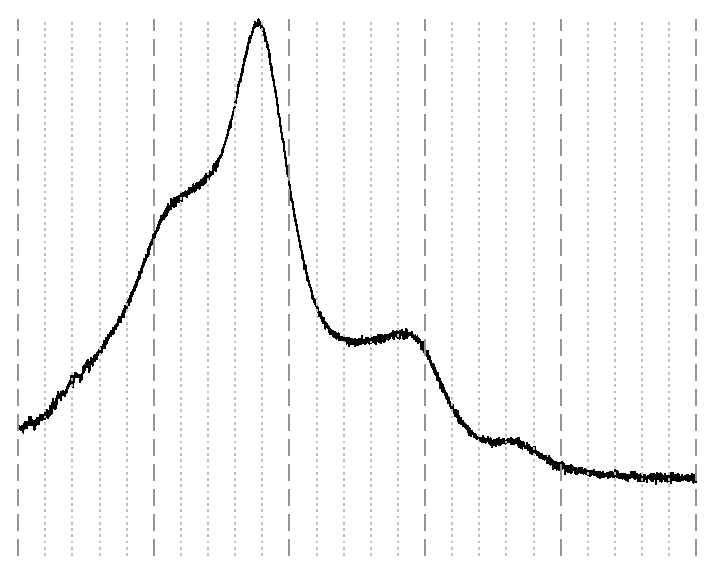
\includegraphics[width=0.95\textwidth,keepaspectratio]{images/b0_peaks/with_B0.eps}
        \caption{Spectral peaks with severe $B_0$ inhomogeneities ($\mu = 175$Hz)}
        \label{subfig:with B0}        
    \end{subfigure}
    \caption{These samples show the effects that can be modeled using the 3D $B_0$ field simulator. In \ref{subfig:without B0}, the spectral peaks have a purely Lorentzian lineshape. In \ref{subfig:some B0}, the lineshape is now Voigtian because the Gaussian term has been added back by the 3D $B_0$ field simulator. In \ref{subfig:with B0}, severe heterogeneities are modeled which produce extremely broad line widths. All three plots use the same x- and y-axes. The observed offsets are caused by the line broadening.}
    \label{fig:B0 effects}
\end{figure}



\begin{figure}[b!]
    \centering
    \begin{tabular}[l]{cc}
    \begin{subfigure}{0.49\textwidth}
        \centering
        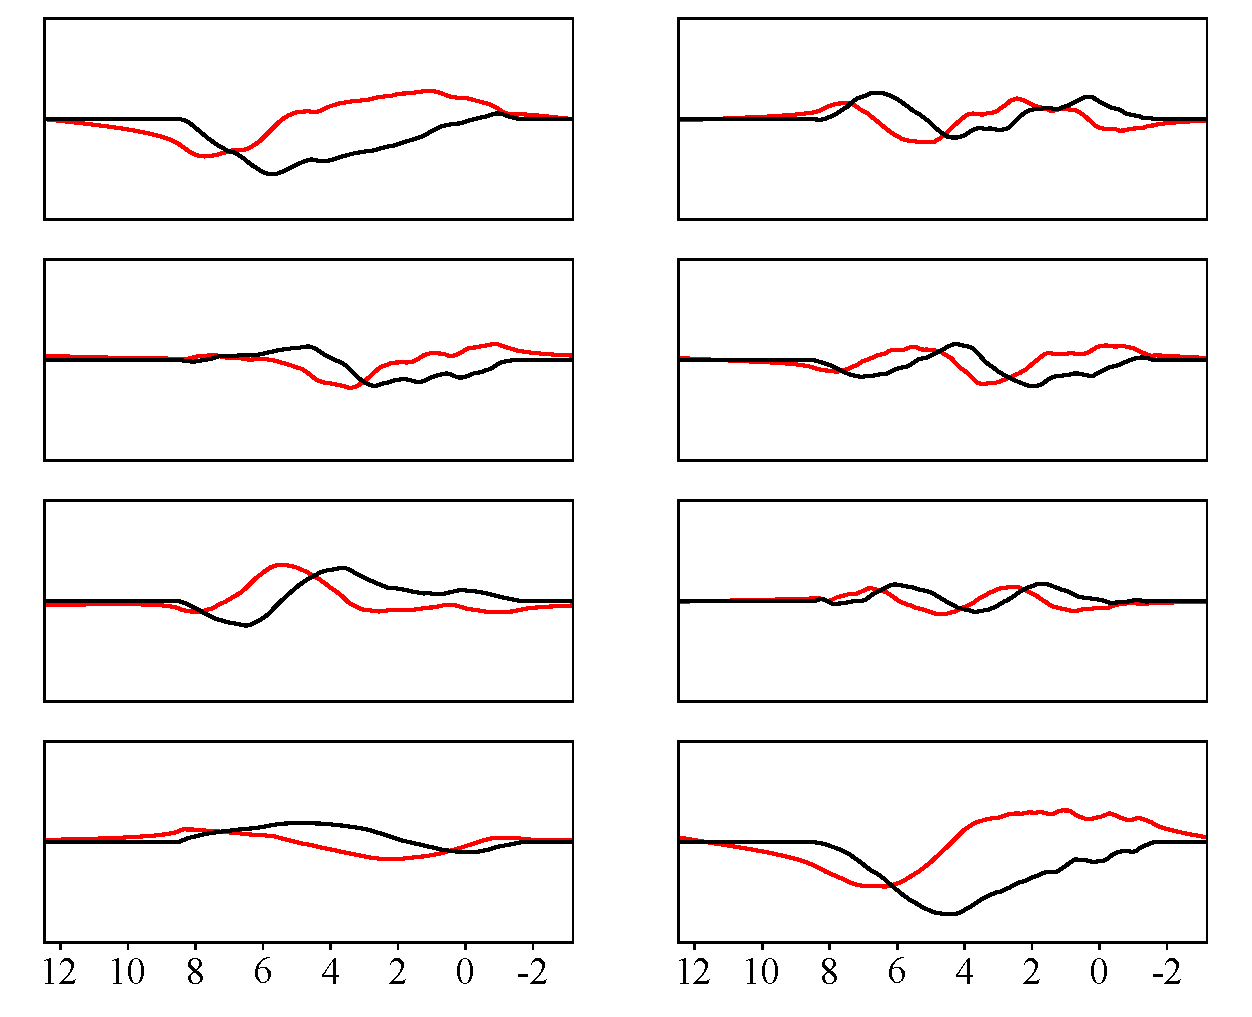
\includegraphics[width=0.95\textwidth,keepaspectratio]{images/random_walks/baseline_walks_edited.eps}
        \caption{Simulated baselines}
        \label{fig:baseline_region}
    \end{subfigure} &
    
    \begin{subfigure}{0.49\textwidth}
        \centering
        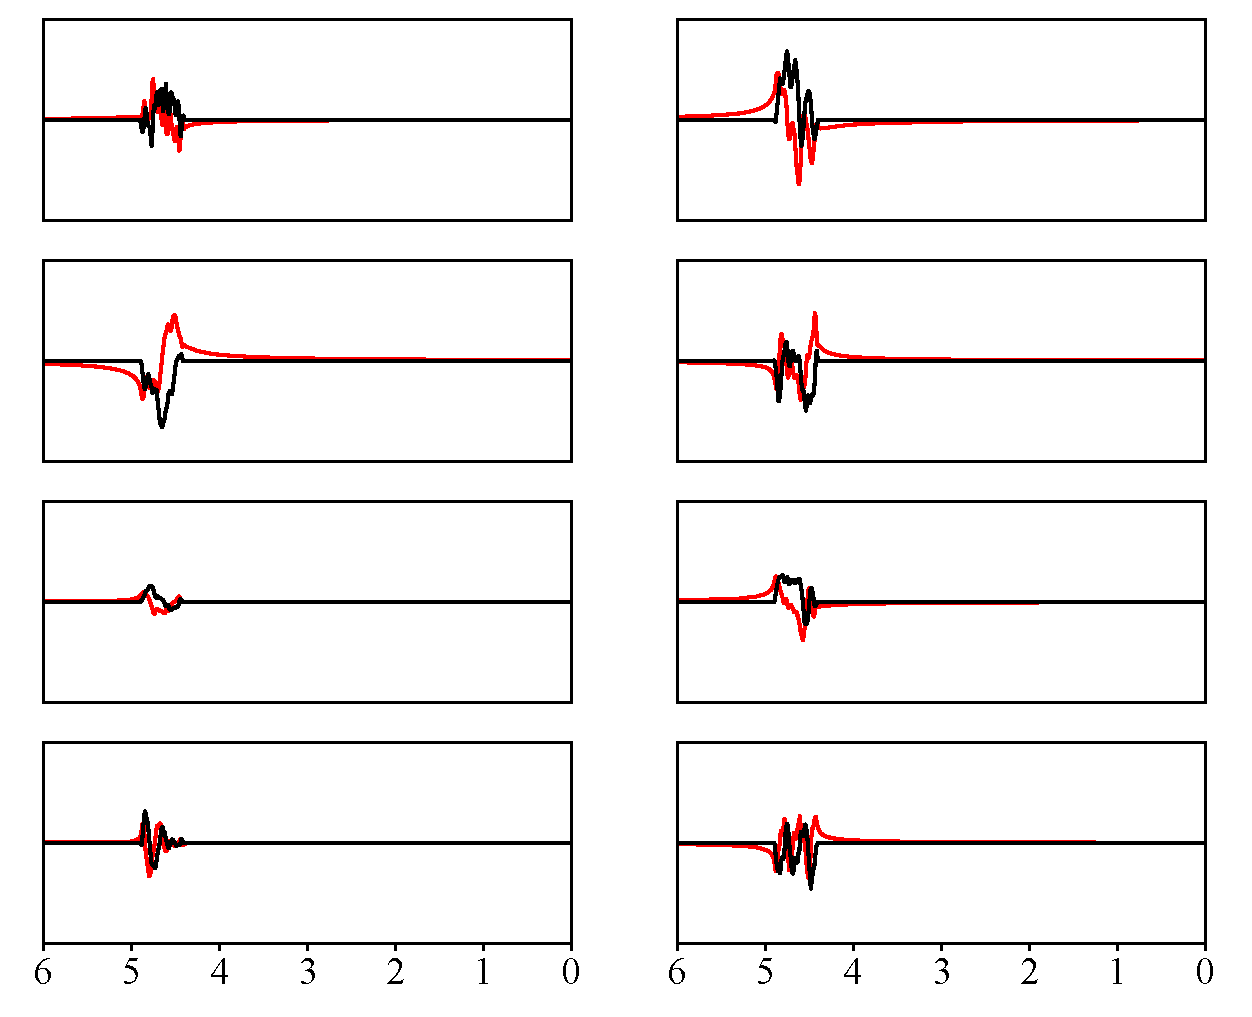
\includegraphics[width=0.95\textwidth,keepaspectratio]{images/random_walks/reswater_walks_edited.eps}
        \caption{Simulated residual water}
        \label{fig:reswater_region}
    \end{subfigure}
    \end{tabular}
    \caption{Simulated  samples of spectral baselines and residual water regions using the pseudo-random bounded walk generator. The blue lines are the raw simulations. The red lines are the smoothed versions that are then returned and applied to the simulated spectra.}
    \label{fig:random walk generator}
\end{figure}



\begin{figure}
    \centering
    \begin{subfigure}{0.32\textwidth}
        \centering
        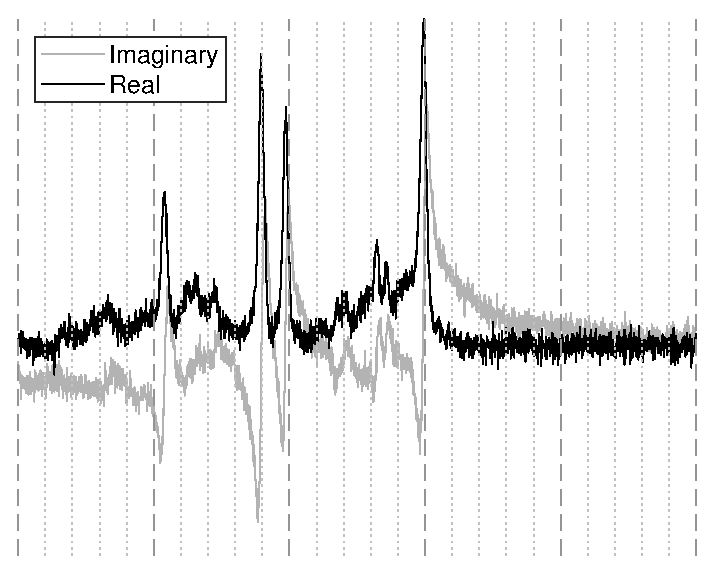
\includegraphics[width=0.95\textwidth,keepaspectratio]{images/phase/no_phase.eps}
        \caption{Spectrum with no phase offsets}
        \label{subfig:no phase}        
    \end{subfigure}
    \begin{subfigure}{0.32\textwidth}
        \centering
        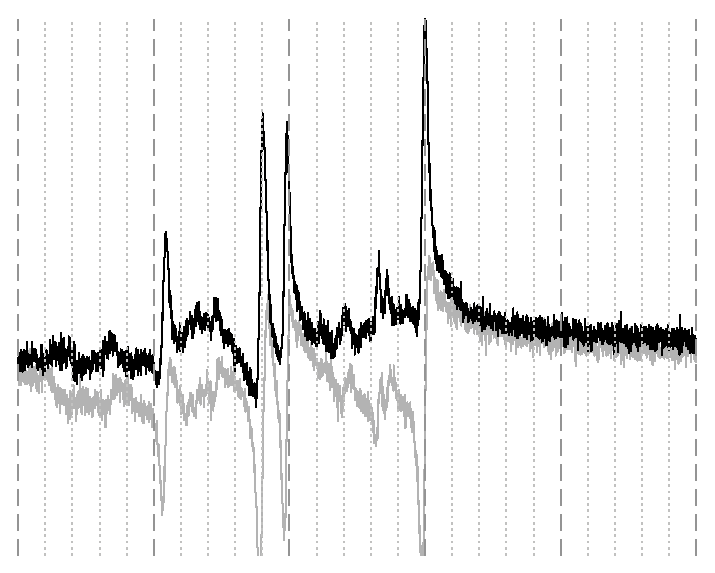
\includegraphics[width=0.95\textwidth,keepaspectratio]{images/phase/zero-order.eps}
        \caption{Spectrum with zero-order phase offset ($\phi_0 = 45^{\circ}$)}
        \label{subfig:zero order phase}        
    \end{subfigure}
    \begin{subfigure}{0.32\textwidth}
        \centering
        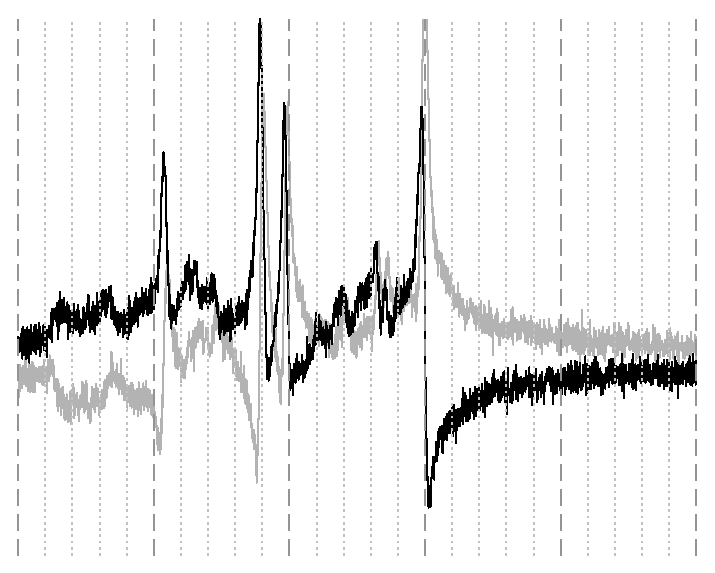
\includegraphics[width=0.95\textwidth,keepaspectratio]{images/phase/first-order.eps}
        \caption{Spectrum with first-order phase offset ($\phi_1 = 20^{\circ}$)}
        \label{subfig:first order phase}        
    \end{subfigure}
    \caption{These samples show how identical spectra are affected by zero- and first-order phase offsets. In \ref{subfig:no phase}, the real component (black) is in absorption mode exhibiting narrow line widths and is fully positive. In \ref{subfig:zero order phase}, a zero-order phase offset is applied. As the spectrum shifts from absorption to dispersion mode, the peaks uniformly lose their symmetry and negative values from the imaginary component are transferred to the real component. In \ref{subfig:first order phase}, a first-order phase shift is applied. This is evident because the asymmetry increases across the spectrum and emanates from the water peak.}
    \label{fig:phase effects}
\end{figure}


\begin{figure}
    \centering
    % \begin{subfigure}{0.32\textwidth}
    %     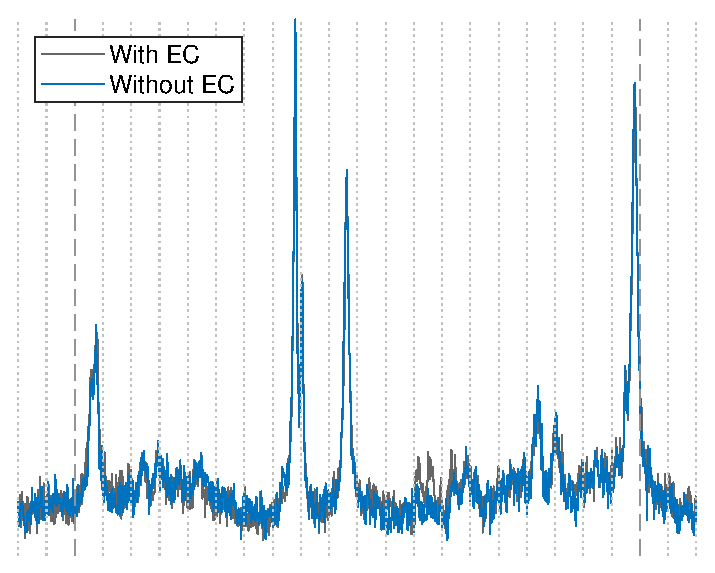
\includegraphics[width=0.95\textwidth, keepaspectratio]{images/eddy/ec=1.eps}
    %     \caption{Eddy current amplitude = 1.0}
    %     \label{subfig:ec=1}        
    % \end{subfigure}
    % \begin{subfigure}{0.32\textwidth}
    %     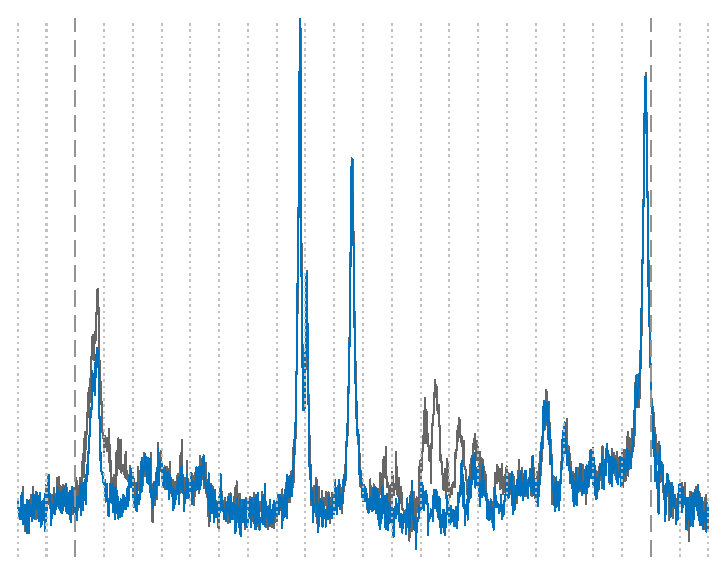
\includegraphics[width=0.95\textwidth, keepaspectratio]{images/eddy/ec=3.eps}
    %     \caption{Eddy current amplitude = 3.0}
    %     \label{subfig:ec=3}        
    % \end{subfigure}
    % \begin{subfigure}{0.32\textwidth}
    %     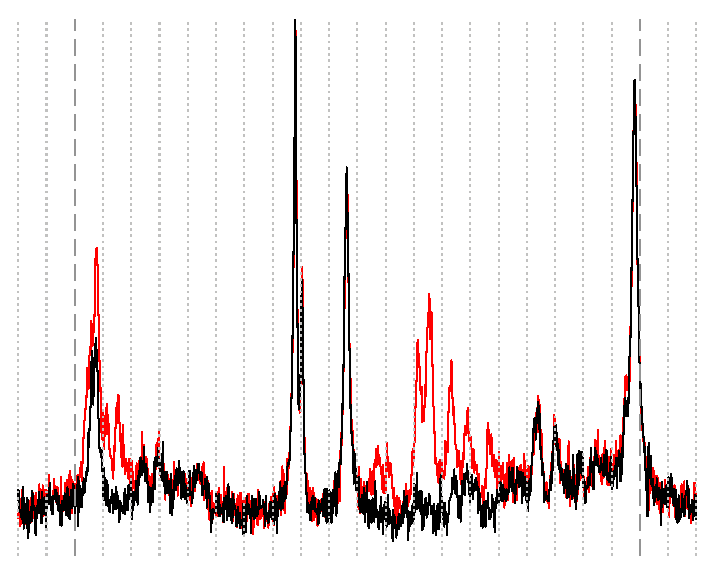
\includegraphics[width=0.95\textwidth, keepaspectratio]{images/eddy/ec=5.eps}
    %     \caption{Eddy current amplitude = 5.0}
    %     \label{subfig:ec=5}        
    % \end{subfigure}
    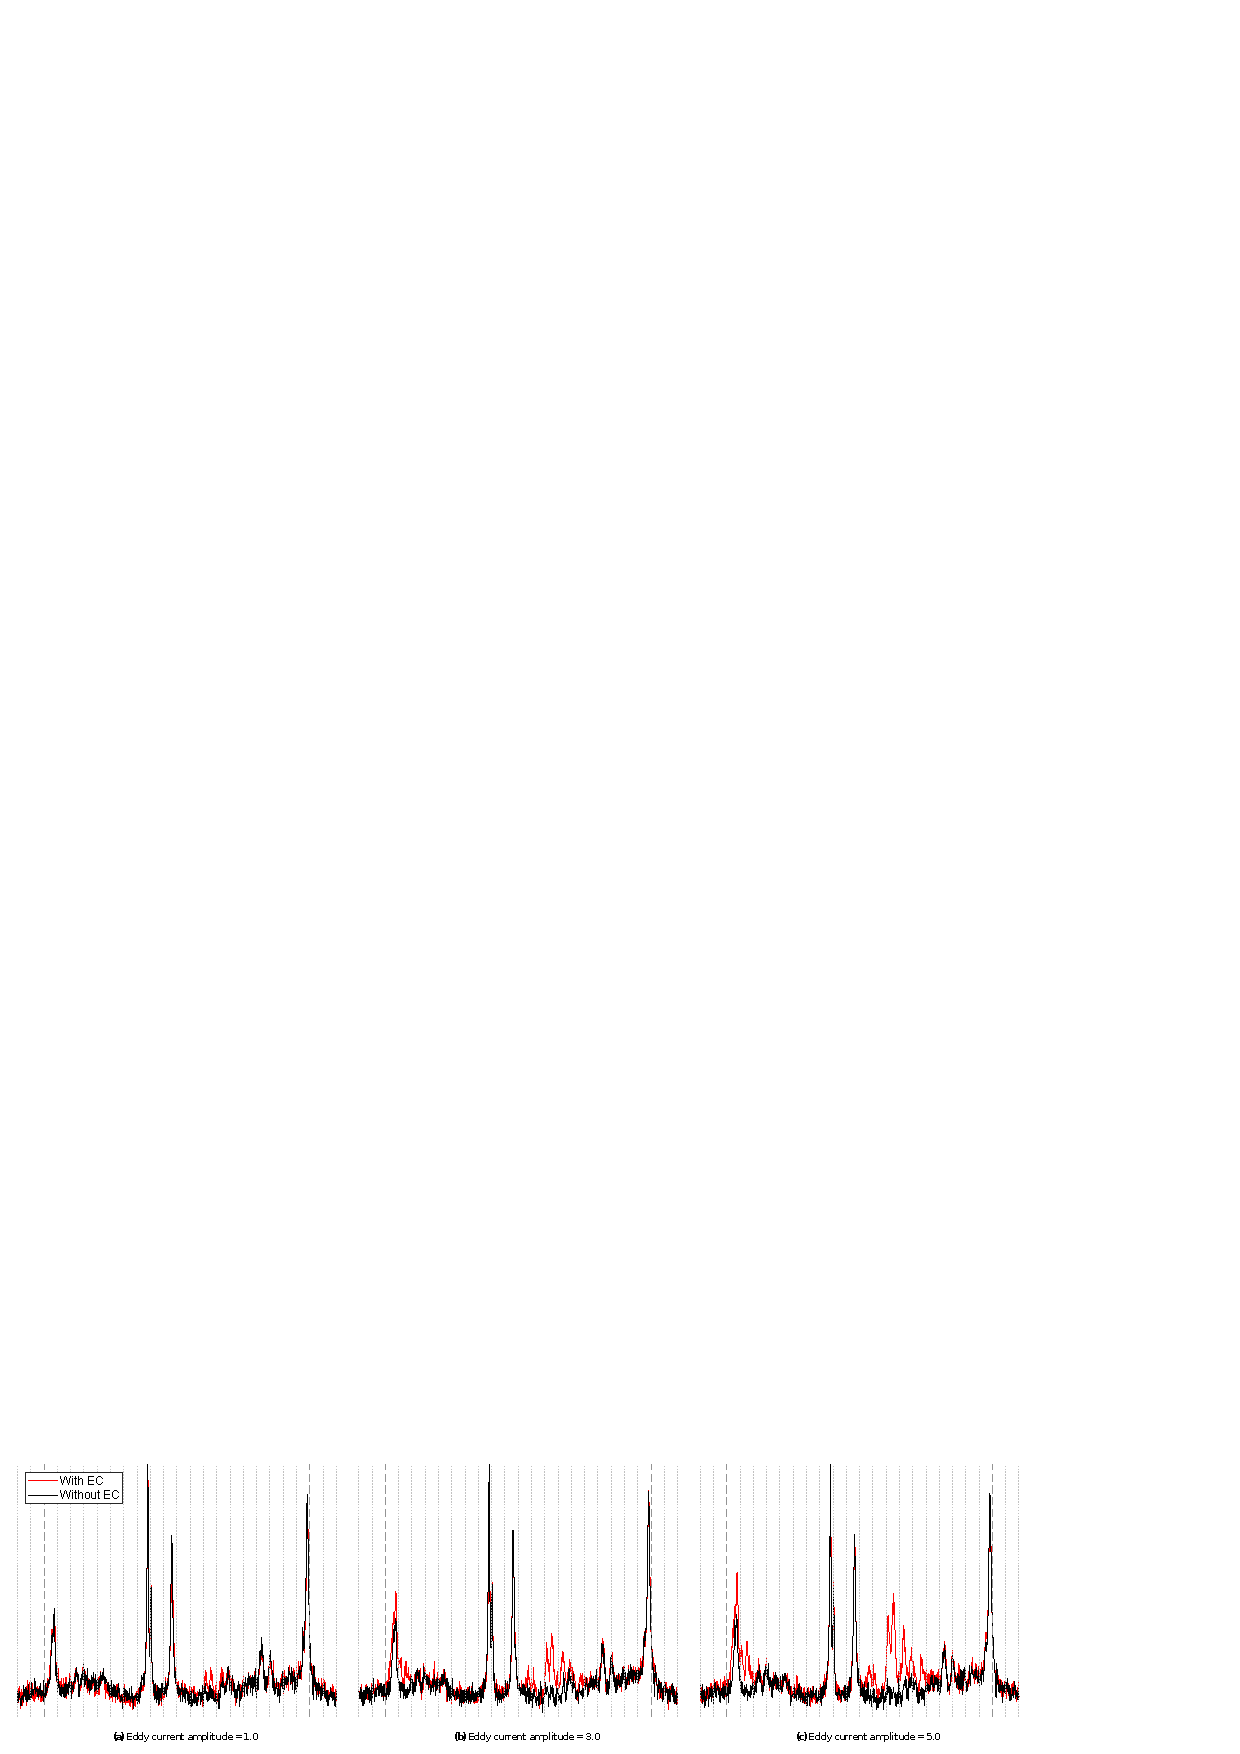
\includegraphics[width=\textwidth,keepaspectratio]{images/compiled_figures/MRS-Sim_Figure6_ eddy_current_effects.png}
    \caption{These 3 samples show the effect of eddy currents on MRS spectra to various degrees. The strength of the eddy currents increases from \ref{subfig:ec=1} to \ref{subfig:ec=5}. If the time constant, $tc$, is set too long, the eddy current artifact will appear as a global frequency shift. In these examples, it can be seen that only some frequencies are affected.}
    \label{fig:eddy currents}
\end{figure}



\begin{figure}[t]
    \centering
    \begin{subfigure}{0.32\textwidth}
        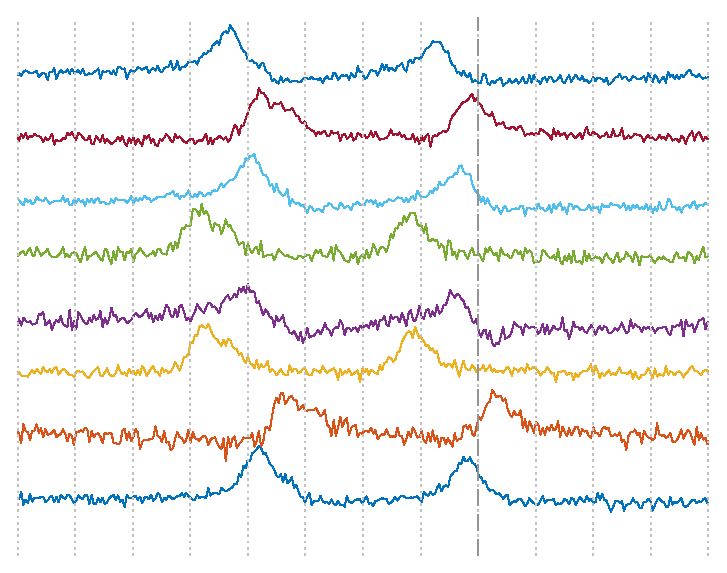
\includegraphics[width=0.95\textwidth, keepaspectratio]{images/samples_transients/8coil_w_phase_w_fshift_cropped.eps}
        \caption{Raw spectral transients}
        \label{subfig:raw transients}        
    \end{subfigure}
    \begin{subfigure}{0.32\textwidth}
        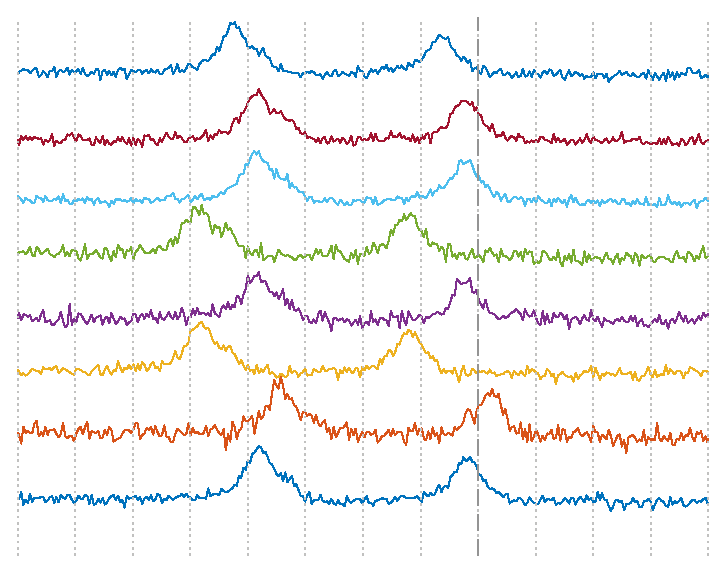
\includegraphics[width=0.95\textwidth, keepaspectratio]{images/samples_transients/8coil_wo_phase_w_fshift_cropped.eps}
        \caption{Phase alignment}
        \label{subfig:phase alignment}        
    \end{subfigure}
    \begin{subfigure}{0.32\textwidth}
        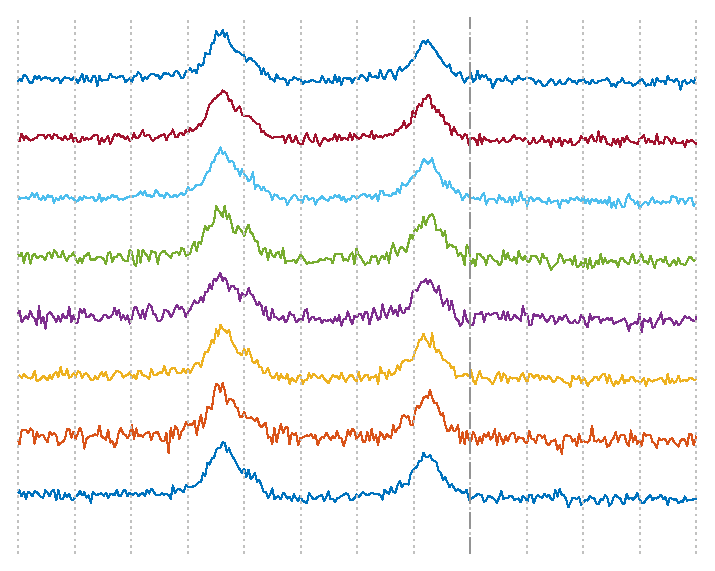
\includegraphics[width=0.95\textwidth, keepaspectratio]{images/samples_transients/8coil_wo_phase_wo_fshift_cropped.eps}
        \caption{Frequency alignment}
        \label{subfig:frequency alignment}        
    \end{subfigure}
    \caption{Examples of 8 simulated coil transients for a 3T GE PRESS sequence with TE=30ms. \ref{subfig:raw transients} shows transients with various SNRs and coil sensitivities along with zero-order phase and frequency offsets. \ref{subfig:phase alignment} shows the transients after phase alignment. \ref{subfig:frequency alignment} shows the transients after frequency alignment. After \ref{subfig:frequency alignment}, the transients can be averaged together and the coil-combined spectrum can then be fitted.}
    \label{fig:simulated transients}
\end{figure}




\subsection{Baseline and Residual Water Generator}\label{resutls:baseline}
\begin{figure}[t!]
    \centering
    \begin{tabular}[c]{ccc}
    \begin{subfigure}[c]{0.31\textwidth}
        \includegraphics[width=0.93\textwidth,keepaspectratio]{images/30ms_samples/curated/30ms_curated_sample{1}.eps}
        \vspace{3pt}
    \end{subfigure}&
    \begin{subfigure}[c]{0.31\textwidth}
        \includegraphics[width=0.93\textwidth,keepaspectratio]{images/30ms_samples/curated/30ms_curated_sample{2}.eps}
        \vspace{3pt}
    \end{subfigure}&
    \begin{subfigure}[c]{0.31\textwidth}
        \includegraphics[width=0.93\textwidth,keepaspectratio]{images/30ms_samples/curated/30ms_curated_sample{3}.eps}
        \vspace{3pt}
    \end{subfigure}\\
    \begin{subfigure}[c]{0.31\textwidth}
        \includegraphics[width=0.93\textwidth,keepaspectratio]{images/30ms_samples/curated/30ms_curated_sample{4}.eps}
        \vspace{3pt}
    \end{subfigure}&
    \begin{subfigure}[c]{0.31\textwidth}
        \includegraphics[width=0.93\textwidth,keepaspectratio]{images/30ms_samples/curated/30ms_curated_sample{5}.eps}
        \vspace{3pt}
    \end{subfigure}&%
    \begin{subfigure}[c]{0.31\textwidth}
        \includegraphics[width=0.93\textwidth,keepaspectratio]{images/30ms_samples/curated/30ms_curated_sample{6}.eps}
        \vspace{3pt}
    \end{subfigure}\\
    \begin{subfigure}[c]{0.31\textwidth}
        \includegraphics[width=0.93\textwidth,keepaspectratio]{images/30ms_samples/curated/30ms_curated_sample{7}.eps}
        \vspace{3pt}
    \end{subfigure}&
    \begin{subfigure}[c]{0.31\textwidth}
        \includegraphics[width=0.93\textwidth,keepaspectratio]{images/30ms_samples/curated/30ms_curated_sample{8}.eps}
        \vspace{3pt}
    \end{subfigure}&
    \begin{subfigure}[c]{0.31\textwidth}
        \includegraphics[width=0.93\textwidth,keepaspectratio]{images/30ms_samples/curated/30ms_curated_sample{9}.eps}
        \vspace{3pt}
    \end{subfigure}\\
    \begin{subfigure}[c]{0.31\textwidth}
        \includegraphics[width=0.93\textwidth,keepaspectratio]{images/30ms_samples/curated/30ms_curated_sample{10}.eps}
        \vspace{3pt}
    \end{subfigure}&
    \begin{subfigure}[c]{0.31\textwidth}
        \includegraphics[width=0.93\textwidth,keepaspectratio]{images/30ms_samples/curated/30ms_curated_sample{11}.eps}
        \vspace{3pt}
    \end{subfigure}&%
    \begin{subfigure}[c]{0.31\textwidth}
        \includegraphics[width=0.93\textwidth,keepaspectratio]{images/30ms_samples/curated/30ms_curated_sample{12}.eps}
        \vspace{3pt}
    \end{subfigure}\\
    \begin{subfigure}[c]{0.31\textwidth}
        \includegraphics[width=0.93\textwidth,keepaspectratio]{images/30ms_samples/curated/30ms_curated_sample{13}.eps}
    \end{subfigure}&
    \begin{subfigure}[c]{0.31\textwidth}
        \includegraphics[width=0.93\textwidth,keepaspectratio]{images/30ms_samples/curated/30ms_curated_sample{14}.eps}
    \end{subfigure}&%
    \begin{subfigure}[c]{0.31\textwidth}
        \includegraphics[width=0.93\textwidth,keepaspectratio]{images/30ms_samples/curated/30ms_curated_sample{15}.eps}
    \end{subfigure}
    \end{tabular}
    \caption{Sample spectra simulated for a PRESS sequence with TE=30ms that highlight the effect of the baseline and residual water contributions.}
    \label{fig:30ms samples curated clean}
\end{figure}

Fig. \ref{fig:30ms samples curated clean} illustrates a single clean short echo (TE=30ms) PRESS spectrum showcasing various combinations of residual water and baseline contributions. The metabolite concentrations and lineshapes were fixed in addition to the settings described above. These samples omit spectral artifacts to more clearly highlight the variety that can be achieved by randomly sampling parameters for the baseline and residual water generator. 

Currently, it is unknown what a true baseline actually looks like. Theory and protocols regarding baseline modeling have been developed extensively, but the physical phenomena underlying the baseline signal is still poorly understood. Different modeling protocols can produce different baselines. Bazgir et al.\cite{Bazgir2018} interpolate between selected minima in the spectra, Wilson et al.\cite{Wilson2021} uses penalized B-splines to overparametize the problem space which is solved using an optimized smoothing constraint, while Osprey\cite{Oeltzschner2020} uses unregularized B-splines spread every 0.4 ppm to enforce smoothness. Even though all of these techniques have been proved useful, in vivo data does not have known ground truths meaning there is no way to identify which method is the most accurate. Without a physics-based model, other methods of baseline simulation are necessary. 

Fig. \ref{fig:30ms samples curated clean} shows a variety of baseline profiles that can be simulated with the presented framework. Instead of claiming to produce in vivo baselines, the proposed generator produces a wide variety of offsets that approximate the baselines extracted by traditional methods. The motivation behind this approach is that if the generator cannot be limited to strictly in vivo-like baselines, then it should incorporate a variety of appropriate baseline profiles such that true baselines are included. Because this generator is not based on a baseline fitting method, future work could use it to evaluate the baseline modeling performance of various fitting protocols given different baseline profiles.


\subsection{Complete Model}\label{results:complete model}
\begin{figure}[ht!]
    \centering
    \begin{tabular}[c]{ccc}
    \begin{subfigure}[c]{0.31\textwidth}
        \includegraphics[width=0.93\textwidth]{images/30ms_samples/dirty/30ms_curated_dirty_sample{1}.eps}
        \vspace{3pt}
    \end{subfigure}&
    \begin{subfigure}[c]{0.31\textwidth}
        \includegraphics[width=0.93\textwidth]{images/30ms_samples/dirty/30ms_curated_dirty_sample{2}.eps}
        \vspace{3pt}
    \end{subfigure}&
    \begin{subfigure}[c]{0.31\textwidth}
        \includegraphics[width=0.93\textwidth]{images/30ms_samples/dirty/30ms_curated_dirty_sample{3}.eps}
        \vspace{3pt}
    \end{subfigure}\\
    \begin{subfigure}[c]{0.31\textwidth}
        \includegraphics[width=0.93\textwidth]{images/30ms_samples/dirty/30ms_curated_dirty_sample{4}.eps}
        \vspace{3pt}
    \end{subfigure}&
    \begin{subfigure}[c]{0.31\textwidth}
        \includegraphics[width=0.93\textwidth]{images/30ms_samples/dirty/30ms_curated_dirty_sample{5}.eps}
        \vspace{3pt}
    \end{subfigure}&%
    \begin{subfigure}[c]{0.31\textwidth}
        \includegraphics[width=0.93\textwidth]{images/30ms_samples/dirty/30ms_curated_dirty_sample{6}.eps}
        \vspace{3pt}
    \end{subfigure}\\
    \begin{subfigure}[c]{0.31\textwidth}
        \includegraphics[width=0.93\textwidth]{images/30ms_samples/dirty/30ms_curated_dirty_sample{7}.eps}
        \vspace{3pt}
    \end{subfigure}&
    \begin{subfigure}[c]{0.31\textwidth}
        \includegraphics[width=0.93\textwidth]{images/30ms_samples/dirty/30ms_curated_dirty_sample{8}.eps}
        \vspace{3pt}
    \end{subfigure}&
    \begin{subfigure}[c]{0.31\textwidth}
        \includegraphics[width=0.93\textwidth]{images/30ms_samples/dirty/30ms_curated_dirty_sample{9}.eps}
        \vspace{3pt}
    \end{subfigure}\\
    \begin{subfigure}[c]{0.31\textwidth}
        \includegraphics[width=0.93\textwidth]{images/30ms_samples/dirty/30ms_curated_dirty_sample{10}.eps}
        \vspace{3pt}
    \end{subfigure}&
    \begin{subfigure}[c]{0.31\textwidth}
        \includegraphics[width=0.93\textwidth]{images/30ms_samples/dirty/30ms_curated_dirty_sample{11}.eps}
        \vspace{3pt}
    \end{subfigure}&%
    \begin{subfigure}[c]{0.31\textwidth}
        \includegraphics[width=0.93\textwidth]{images/30ms_samples/dirty/30ms_curated_dirty_sample{12}.eps}
        \vspace{3pt}
    \end{subfigure}\\
    \begin{subfigure}[c]{0.31\textwidth}
        \includegraphics[width=0.93\textwidth]{images/30ms_samples/dirty/30ms_curated_dirty_sample{13}.eps}
    \end{subfigure}&
    \begin{subfigure}[c]{0.31\textwidth}
        \includegraphics[width=0.93\textwidth]{images/30ms_samples/dirty/30ms_curated_dirty_sample{14}.eps}
    \end{subfigure}&%
    \begin{subfigure}[c]{0.31\textwidth}
        \includegraphics[width=0.93\textwidth]{images/30ms_samples/dirty/30ms_curated_dirty_sample{15}.eps}
    \end{subfigure}\\
    \end{tabular}
    \caption{Sample spectra, similar to Fig. \ref{fig:30ms samples curated clean} [PRESS, TE=30ms], with randomly sampled, uncorrected artifacts to approximate raw data.}%Sample spectra simulated for a PRESS sequence with TE=30ms. These spectra have sampled parameters just like Fig. \ref{fig:30ms samples curated clean} plus a variety of uncorrected artifacts including eddy currents, zero- and first-order phase offsets, frequency shifts, macromolecule and lipid contributions, residual water, and baseline offsets.}
    \label{fig:30ms samples curated dirty}
\end{figure}


In contrast, Fig. \ref{fig:30ms samples curated dirty} presents a simulated PRESS spectrum (TE=30ms) with randomly sampled artifacts and offsets. This figure highlights the variety a single spectrum can assume just by randomly sampling the artifacts. Sophisticated simulations, such as these, are useful for developing and validating data processing techniques such as artifact removal and new spectral fitting protocols. Spectra can be simulated to be as clean or as artifact-laden as desired, all while maintaining known ground truth values. 


Upon closer inspection of Fig. \ref{fig:30ms samples curated dirty}, the baselines and residual water regions sometimes appear to be uncorrelated with the depicted spectra, but they are in fact paired. These discrepancies are due to the additional artifacts that are applied to the simulations after all of the spectral components are combined. The plotted baseline and residual water regions are the ground truth signals and do not have other artifacts applied to them. 

Incorporating a robust collection of artifacts and phenomena commonly encountered with in vivo data into these simulations, makes resulting datasets more closely approximate raw, in vivo data. Even though post-processing techniques are highly accurate, they have limitations and biases, leaving some residue of the corrected artifacts. Including these artifacts in the simulations and removing them with the users' own post-processing and fitting protocols ensures consistency between simulated and in vivo data. These artifacts can also be scaled down in the simulations to emulate residual artifacts. However, this is not ideal because it cannot be guaranteed that scaling down the artifacts will accurately reflect the biases and residues found in the in vivo data.


Deep learning techniques also benefit from robust and consistent synthetic data. Ensuring consistency of the synthetic training data with the in vivo data promotes better model performance. While including fine-grained detail, such as sampling moiety-level T2 values, may not be essential for every use case, in a deep learning setting, it acts as a form of data augmentation. Data augmentation techniques maintain the underlying data but manipulate its appearance so that models learn a broader range of features instead of overfitting a single pattern. Such techniques are standard practice in deep learning and are an inherent feature of this framework. 

